\renewcommand{\thesection}{\Roman{section}}
\titleformat{\section}
{\normalfont\bfseries}{PHẦN~\thesection.}{0.4em}{}
\newcolumntype{C}[1]{>{\centering\arraybackslash}p{#1}}
\newcolumntype{L}[1]{>{\raggedright\arraybackslash}p{#1}}
\begin{tabular}{C{5cm}C{11cm}}
	\textbf{TRUNG TÂM MANABIE}& \textbf{ĐỀ ÔN TẬP KIỂM TRA GIỮA HỌC KÌ 2} \\
	\textbf{ĐỀ 05}& \textbf{Môn: VẬT LÝ}\\
	\textit{(Đề có 02 trang)}& \textit{Thời gian làm bài: 50 phút, không kể thời gian phát đề}
	
	\noindent\rule{4cm}{0.8pt} \\
\end{tabular}
\begin{enumerate}[label=\bfseries Câu \arabic*:]
	\item \textit{(1,5 điểm)} Hình \ref{fig:5} là một bạn nữ sinh đang chạm tay vào máy phát tĩnh điện.
	\begin{center}
		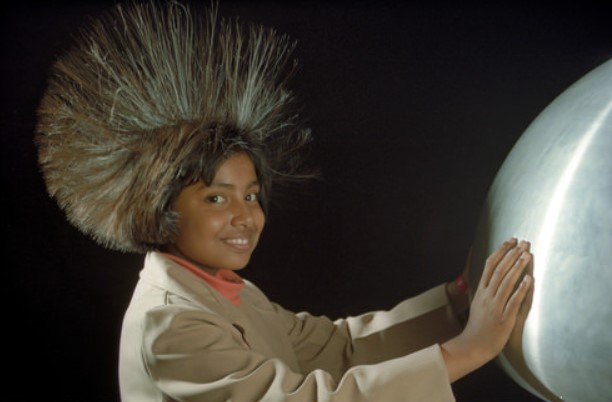
\includegraphics[width=0.35\linewidth]{../figs/PH11-MidSem2-05-5}
		\captionof{figure}{}
		\label{fig:5}
	\end{center}
	\begin{enumerate}[label=\alph*)]
		\item Tại sao tóc của bạn nữ sinh lại dựng đứng lên?
		\item Theo em, chân bạn nữ sinh có chạm vào đất không? Giải thích vì sao.
	\end{enumerate}
\hideall{
\begin{enumerate}[label=\alph*)]
	\item Khi bạn nữ sinh chạm vào máy phát tĩnh điện thì bạn nữ sinh nhiễm điện cùng dấu với máy phát. Do các sợi tóc của bạn nữ sinh nhiễm điện cùng dấu nên chúng đẩy nhau và gây ra hiện tượng như được mô tả ở đề bài.
	\item Chân bạn nữ sinh không chạm đất. Nếu chân bạn chạm đất bạn sẽ được trung hoà điện do điện tích của bạn sẽ trung hoà với điện tích của mặt đất.
\end{enumerate}
}
	\item \textit{(1,5 điểm)} Một proton được tăng tốc từ trạng thái nghỉ trong điện trường đều có độ lớn cường độ điện trường $\SI{640}{\newton/\coulomb}$. Sau một khoảng thời gian $\Delta t$, proton đạt tốc độ $\SI{1.20E6}{\meter/\second}$. Khối lượng của proton là $m_p=\SI{1.67E-27}{\kilogram}$.
	\begin{enumerate}[label=\alph*)]
		\item Xác định độ lớn gia tốc trong chuyển động của proton.
		\item Xác định giá trị $\Delta t$.
		\item Proton phải dịch chuyển quãng đường bao xa để đạt được tốc độ trên?
	\end{enumerate}
\hideall{
\begin{enumerate}[label=\alph*)]
	\item Gia tốc trong chuyển động của proton:
	$$a=\dfrac{F_\text{đ}}{m_p}=\dfrac{\left|q\right|E}{m_p}\approx\SI{6.13E10}{\meter/\second^2}.$$
	\item Khoảng thời gian chuyển động của proton:
	$$\Delta t=\dfrac{v}{a}\approx\SI{1.96E-5}{\second}.$$
	\item Quãng đường proton dịch chuyển:
	$$s=\dfrac{m_pv^2}{2qE}\approx\SI{11.74}{\meter}.$$
\end{enumerate}
}

	\item \textit{(2,0 điểm)} Một quả cầu nhỏ tích điện $q=\SI{68}
{\micro\coulomb}$ và có khối lượng $m=\SI{5.8}{\gram}$ được nối với tường bằng sợi dây nhẹ. Hệ được đặt trong điện trường đều có vector cường độ điện trường $\vec{E}$ hợp với phương ngang góc $\theta=\SI{37}{\degree}$. Quả cầu đạt trạng thái cân bằng tĩnh khi dây treo có phương nằm ngang như hình vẽ \ref{fig:1}. Lấy $g=\SI{10}{\meter/\second^2}$.
\begin{center}
	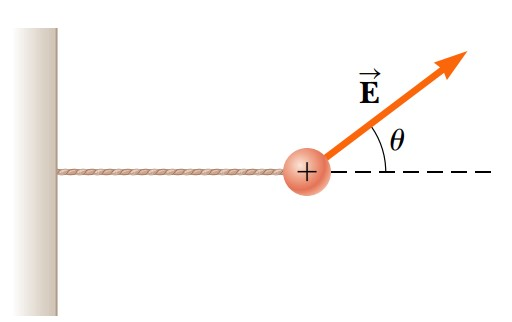
\includegraphics[width=0.35\linewidth]{../figs/PH11-MidSem2-05-1}
	\captionof{figure}{}
	\label{fig:1}
\end{center}
\begin{enumerate}[label=\alph*)]
	\item Vẽ hình, phân tích các lực tác dụng lên quả cầu. Tính độ lớn lực tĩnh điện tác dụng lên quả cầu.
	\item Tính độ lớn lực căng của dây.
\end{enumerate}
\hideall{
\begin{enumerate}
	\item Quả cầu chịu tác dụng của các lực: trọng lực $\vec{P}$, lực căng dây $\vec{T}$, lực tĩnh điện $\vec{F}_\text{đ}$.
	\begin{center}
		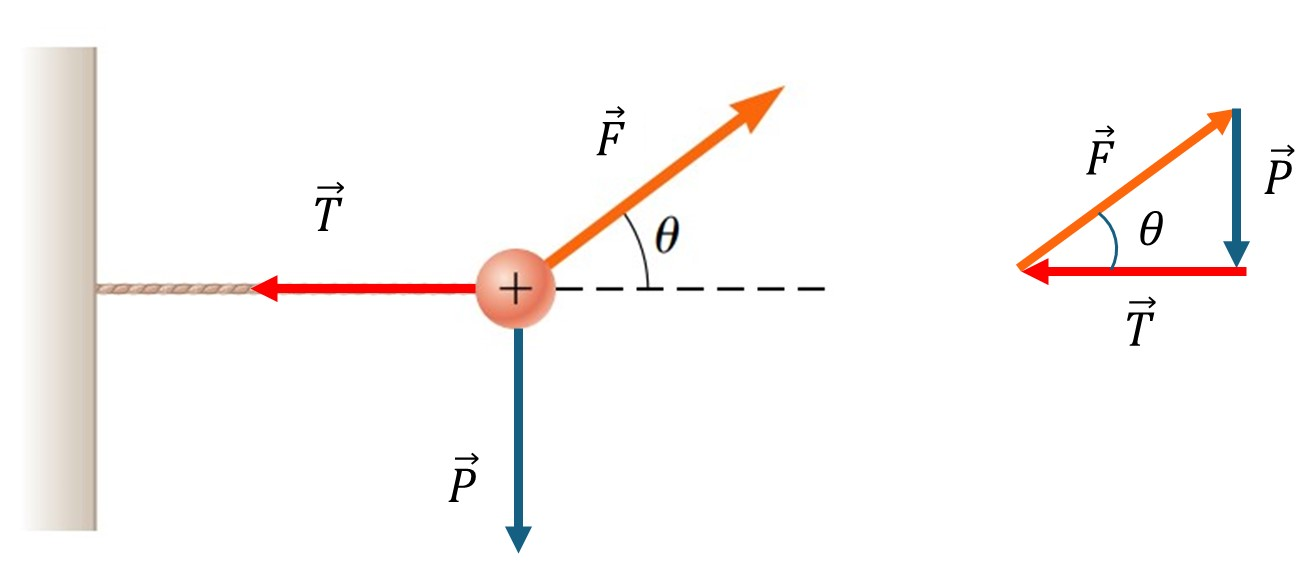
\includegraphics[width=0.7\linewidth]{../figs/PH11-MidSem2-05-6}
	\end{center}
Quả cầu cân bằng nên $\vec{P}+\vec{T}+\vec{F}_\text{đ}=\vec{0}$.\\
Ta có:
$$F_\text{đ}=\dfrac{mg}{\sin\theta}\approx\SI{0.096}{\newton}.$$
\item Độ lớn lực căng dây:
$$T=\dfrac{mg}{\tan\theta}\approx\SI{0.077}{\newton}.$$
\end{enumerate}
}


\item \textit{(1,5 điểm)} Hai điện tích điểm dương, hoàn toàn giống nhau được đặt tại hai đỉnh của hình thang cân như hình vẽ \ref{fig:2}. Xác định biểu thức cường độ điện trường tổng hợp do hai điện tích gây ra tại P.
\begin{center}
	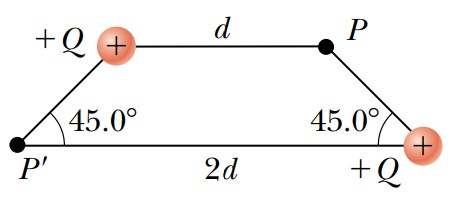
\includegraphics[width=0.35\linewidth]{../figs/PH11-MidSem2-05-2}
	\captionof{figure}{}
	\label{fig:2}
\end{center}
\hideall{
\begin{center}
	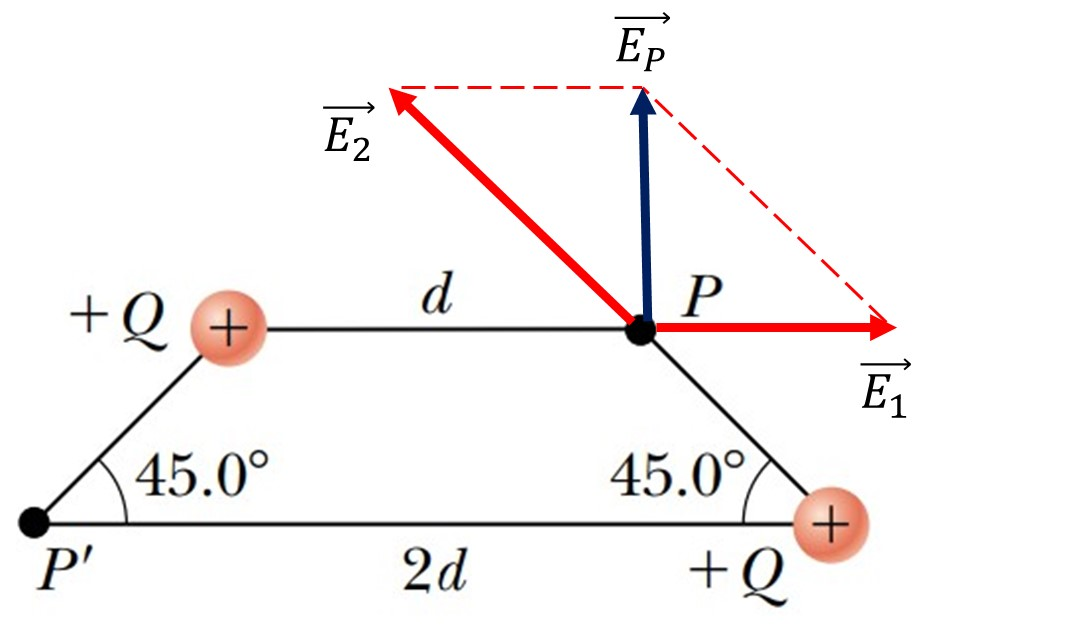
\includegraphics[width=0.5\linewidth]{../figs/PH11-MidSem2-05-7}
\end{center}
$$r_1=d; \quad r_2=\dfrac{0,5d}{\cos\SI{45}{\degree}}=\dfrac{d\sqrt{2}}{2}.$$
Cường độ điện trường do mỗi điện tích gây ra tại P:
$$\begin{cases}
	E_1=\dfrac{kQ}{\varepsilon r^2_1}=\dfrac{kQ}{\varepsilon d^2}\\
	E_2=\dfrac{kQ}{\varepsilon r^2_2}=\dfrac{kQ}{\varepsilon \left(\dfrac{d\sqrt{2}}{2}\right)^2}=\dfrac{2kQ}{\varepsilon d^2}
\end{cases}$$
Cường độ điện trường tổng hợp tại P:
$$\vec{E}_\text{P}=\vec{E}_1+\vec{E}_2$$
Do $\left(\vec{E}_1, \vec{E}_1\right)=\SI{135}{\degree}$
$$E_\text{P}=\sqrt{E^2_1+E^2_2+2E_1E_2\cos\SI{135}{\degree}}\approx\dfrac{1,47kQ}{\varepsilon d^2}.$$
}

\item \textit{(2,0 điểm)} Trong điện trường đều cho ba điểm A, B, C tao thành tam giác vuông tại C. Trong đó $\text{AC}=\SI{4}{\centi\meter}$, $\text{BC}=\SI{3}{\centi\meter}$. Vector cường độ điện trường $\vec{E}$ song song với AC và có độ lớn $E=\SI{2E4}{\volt/\meter}$.
\begin{center}
	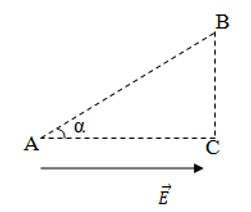
\includegraphics[width=0.3\linewidth]{../figs/PH11-MidSem2-05-4}
	\captionof{figure}{}
\end{center}
\begin{enumerate}[label=\alph*)]
	\item Tính hiệu điện thế $U_\text{AC}$, $U_\text{AB}$, $U_\text{BC}$.
	\item Tính công của lực điện trường khi một electron di chuyển từ A đến B.
\end{enumerate}
\hideall{
\begin{enumerate}[label=\alph*)]
	\item	\begin{eqnarray*}
		U_\text{AC}&=&Ed_\text{AC}=E\cdot AC \cos\SI{0}{\degree}=\SI{800}{\volt}\\
		U_\text{AB}&=&Ed_\text{AB}=E\cdot AC=\SI{800}{\volt}\\
		U_\text{BC}&=&Ed_\text{BC}=\SI{0}{\volt}.
	\end{eqnarray*}
\item $A_\text{AB}=qU_\text{AB}=\SI{-1.28E-16}{\joule}$.
\end{enumerate}
}

\item \textit{(1,5 điểm)} Bốn tụ điện được nối với acquy như sơ đồ hình \ref{fig:3}. 
\begin{center}
	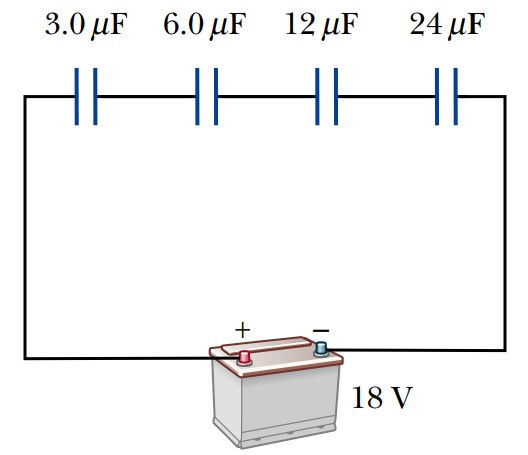
\includegraphics[width=0.35\linewidth]{../figs/PH11-MidSem2-05-3}
	\captionof{figure}{Bốn tụ điện được nối với acquy}
	\label{fig:3}
\end{center}
\begin{enumerate}[label=\alph*)]
	\item Tính điện dung của bộ tụ điện.
	\item Tính điện tích mà tụ $\SI{12}{\micro\farad}$ tích được.
	\item Tính hiệu điện thế hai đầu tụ $\SI{12}{\micro\farad}$.
\end{enumerate}
\hideall{
\begin{enumerate}[label=\alph*)]
	\item Do các tụ ghép nối tiếp nhau nên điện dung của bộ tụ điện:
	$$\dfrac{1}{C_b}=\dfrac{1}{C_1}+\dfrac{1}{C_2}+\dfrac{1}{C_3}+\dfrac{1}{C_4}\Rightarrow C_b=\SI{1.6}{\micro\farad}.$$
	\item Điện tích tụ $\SI{12}{\micro\farad}$ tích được:
	$$Q_3=C_bU=\left(\SI{1.6}{\micro\farad}\right)\cdot\left(\SI{18}{\volt}\right)=\SI{29}{\micro\coulomb}.$$
	\item Hiệu điện thế giữa hai bản tụ điện $\SI{12}{\micro\farad}$:
	$$U_3=\dfrac{Q_3}{C_3}=\dfrac{\SI{29}{\micro\coulomb}}{\SI{12}{\micro\farad}}=\SI{2.4}{\volt}.$$
\end{enumerate}
}

\end{enumerate}
\begin{center}
	\textbf{--- HẾT ---}
\end{center}
